\documentclass[11pt, oneside]{article} 
\usepackage{geometry}
\geometry{letterpaper} 
\usepackage{graphicx}
	
\usepackage{amssymb}
\usepackage{amsmath}
\usepackage{parskip}
\usepackage{color}
\usepackage{hyperref}

\graphicspath{{/Users/telliott_admin/Tex/png/}}
% \begin{center} 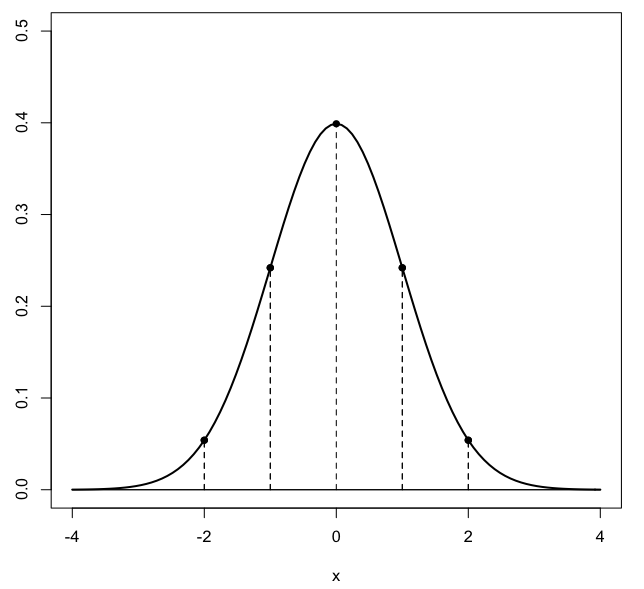
\includegraphics [scale=0.4] {gauss3.png} \end{center}

%break
\title{Sum of angles}
\date{}

\begin{document}
\maketitle
\Large

\label{sec:sum_angles_distance}

\subsection*{Strang}

For a geometric derivation of the sum of angles formula with minimal setup, I really like this figure from Strang

\begin{center} 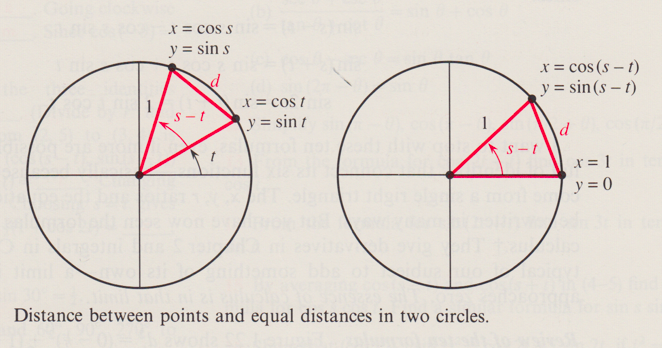
\includegraphics [scale=0.6] {strang_sum.png} \end{center}

We have the same triangle in the two panels, just rotated clockwise on the right.

To compute the distance between two points in the plane we do
\[ d = \sqrt{(x_2 - x_1)^2 + (y_2 - y_1)^2} \]
(This is just the Pythagorean theorem in disguise).

We don't actually need to take the square root, let's stick with
\[ d^2 = (x_2 - x_1)^2 + (y_2 - y_1)^2 \]

In the first figure, $t$ is the angle between the lower radius and the $x$-axis, $s$ is the angle between the upper radius and the $x$-axis, and as labeled, $s-t$ is the angle between the two radii.

The distance $d$ squared for the left panel is
\[ d^2 = (\cos s - \cos t)^2 + (\sin s - \sin t)^2 \]

Multiply out:
\[ d^2 = \cos^2 s - 2 \cos s \cos t  + \cos^2 t +  \sin^2 s - 2 \sin s \sin t + \sin^2 t \]
We have two copies of $\sin^2 + \cos^2$, one for angle $s$  and one for $t$
\[ d^2 = 2 - 2 \cos s \cos t - 2 \sin s \sin t \]

In the right panel, the two radii have been rotated, preserving the same angle between them.
\[  d^2 = (\cos (s-t) - 1)^2 + \sin(s-t)^2 \]
(Don't forget the $1$).
\[ = \cos^2 (s-t) - 2 \cos(s-t) + 1 + \sin^2 (s-t) \]
\[ = 2 - 2 \cos(s-t) \]

Because the included angle hasn't changed, neither has the distance, so we can equate the two expressions.  
\[ 2 - 2 \cos(s-t) = 2 - 2 \cos s \cos t - 2 \sin s \sin t \]
Subtract 2 from both sides, multiply by $1/2$, and change sign to give
\[ \cos (s - t) = \cos s \cos t + \sin s \sin t \]
This is our first formula, for the cosine of the difference of two angles.

\subsection*{getting to sine}

Look at the relationships between sine and cosine for angles that are related by addition or subtraction of $\pi/2$.
\begin{center} 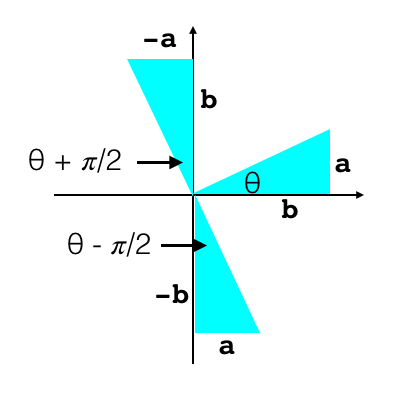
\includegraphics [scale=0.4] {angles2.png} \end{center}
In the figure, I have simply rotated the same triangle.

From the figure we can easily read off these four identities
\[ \sin (\theta + \pi/2) = b = \cos \theta \]
\[ \cos (\theta + \pi/2) = -a = -\sin \theta \]
And
\[ \sin (\theta - \pi/2) = - b = -\cos \theta \]
\[ \cos (\theta - \pi/2) = a = \sin \theta \]

Here is an alternative derivation which proceeds from the graph of sine and cosine versus the angle.

\begin{center} 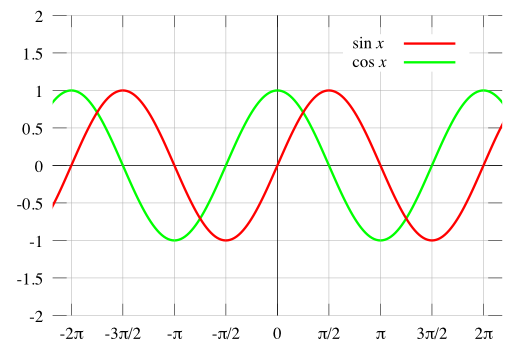
\includegraphics [scale=0.4] {sine_cosine_wikipedia.png} \end{center}

Pick some angle (say $\theta = 0$), then $\cos \theta = 1$.  What is the angle for which the sine gives the same result?  The sine curve is exactly like the cosine, it is just shifted to the right by a \emph{phase change} of $\pi/2$. 

That angle is $\theta + \pi/2$.  The phase change is added to the angle:
\[ \cos \theta = \sin (\theta + \frac{\pi}{2}) \]

Try the same reasoning in reverse.

The cosine curve is exactly like the sine, it is just shifted by a phase change of $-\pi/2$, i.e. to the left.  Pick some angle (say $\theta = \pi/2$), then $\sin \theta = 1$.  What is the value of the angle for which the cosine gives the same result?  

It is $\theta - \pi/2$.  The phase change is subtracted from the angle $\theta$:
\[ \sin \theta = \cos (\theta - \frac{\pi}{2}) \]

In summary, switching sine for cosine gives a valid expression, but there is a difference of \emph{sign} for the phase.

\subsection*{back to our task}

So our sum of angles formula (well, really, the difference of angles) was
\[ \cos (s - t) = \cos s \cos t + \sin s \sin t \]
Let
\[ u = t - \frac{\pi}{2} \]
\[ t  = u + \frac{\pi}{2} \]

Substitute for $t$
\[ \cos \ [ \ s - (u + \frac{\pi}{2}) \ ] \ = \cos s \cos (u + \frac{\pi}{2}) + \sin s \sin (u + \frac{\pi}{2}) \]
Regroup the left-hand side
\[ \cos \ [ \ (s - u) - \frac{\pi}{2}) \ ] \ = \cos s \cos (u + \frac{\pi}{2}) + \sin s \sin (u + \frac{\pi}{2}) \]

Referring to the results we obtained above, cosine something minus $\pi/2$ is the sine of that something:
\[ \sin (s - u) = \cos s \cos (u + \frac{\pi}{2}) + \sin s \sin (u + \frac{\pi}{2}) \]
Cosine something plus $\pi/2$ is minus the sine:
\[ \sin (s - u) = -\cos s \sin u + \sin s \sin (u + \frac{\pi}{2}) \]
Sine something plus $\pi/2$ is cosine:
\[ \sin (s - u) = -\cos s \sin u + \sin s \cos u \]

Rearrange:
\[ \sin (s - u) = \sin s \cos u - \sin u \cos s \]

This is correct, but the path is fraught with error!  

For now, memorize. Soon we will see a very simple and effective \hyperref[sec:Euler_sum_angles]{\textbf{aid to memory}} due to Euler.

\subsection*{sum of tangents}

It is also easy to derive the sum of tangents from the sum of sines and cosines.
\[ \tan s + t = \frac{\sin s + t}{\cos s + t} \]
\[ = \frac{\sin s \cos t + \cos s \sin t}{\cos s \cos t - \sin s \sin t} \]
Divide by $\cos s \cos t$
\[ \tan s + t = \frac{\tan s + \tan t}{1 - \tan s \tan t} \]
\[ \tan s - t = \frac{\tan s - \tan t}{1 + \tan s \tan t} \]

We will use these for a few problems later in the book.

\end{document}